
Se comienza el trabajo en el laboratorio y con la intención de probar nuestras habilidades básicas. En particular se presenta como objetivo el enseñar, prácticar y cálcular el error respectivo del uso de las micropipetas (semejante a la mostrada en la Fig. \ref{pipeta})

\textbf{\textcolor{azul50}{Formalismo}}

Desde hace muchos años se ha usado el color como ayuda para reconocer las sustancias químicas; al  reemplazar  el  ojo  humano  por  otros  detectores  de  radiación  se  puede  estudiar  la  absorción  de sustancias, no solamente en la zona del espectro visible, sino también en ultravioleta e infrarrojo. 

Se  denomina  espectrofotometría  a  la  medición  de  la  cantidad  de  energía  radiante  que  absorbe  un sistema  químico  en  función  de  la  longitud  de  onda  de  la  radiación,  y  a  las  mediciones  a  una determinada longitud de onda, esta técnica comprende una serie de técnicas analíticas usadas para el análisis. Las moléculas tienen un estado energético que se puede alterar por la absorción de radiación electromagnética a determinada longitud de onda, lo que se puede medir para realizar un estudio cualitativo o cuantitativo. Las principales ventajas de la espectrofotometría son:\\[-.6cm]
\begin{itemize}
    \item Sensibilidad relativa elevada.\\[-.6cm]
    \item Facilidad para realizar mediciones rápidas.\\[-.6cm]
    \item Grado de especificidad relativamente elevado. 
\end{itemize}
Para obtener la máxima sensibilidad en una determinación debe conocerse la longitud de onda de mayor absorción de la sustancia analizada, que no deberá coincidir con una alta absorción de otras sustancias presentes en la reacción.
Cuando una radiación electromagnética de intensidad $I$ atraviesa un medio homogéneo, parte de la radiación es absorbida por la muestra y otra parte es transmitida con una intensidad $i$, de tal manera que se define transmitancia de una muestra como la relación entre la radiación transmitida $i$ vs $I$, multiplicado $\times 100$: 
\begin{equation}
    T^{(\%)} = \dfrac{i}{I}\times 100
\end{equation}
La absorbancia es una medida de la cantidad de Energía luminosa incidente absorbida por una sustancia en solución. Está relacionada con Transmitancia por medio de : 
\begin{equation}
    A=-\log T = \log T^{(\%)}/100
\end{equation}
La Ley de Lambert y Beer expresa que la absorbancia de una solución es directamente proporcional al camino recorrido por la radiación electromagnética y a la concentración de la
solución. 
\begin{equation}
    A = abc
    \label{ley}
\end{equation}
donde tenemos que, $A$ es la absorbancia, $a$ es la absortividad específica de cada soluto, $b$ es distancia recorrida por el haz de luz en $cm$, $c$ la concentración de la solución. En específico la absortividad es la constante de proporcionalidad que nos permite igualar la ecuación, sus unidades dependerán de $b$ y $c$, ya que la absorbancia no tiene unidades; si $b$ está en $cm$ y $c$ en moles por $litro$, la absortividad estará en $litros\cdot cm~/~ mol $ 
y se denomina coeficiente de absorción molar .

Esta ley permite establecer una relación lineal entre absorbancia y concentraciones de una especie absorbente a una temperatura dada, no se conocen excepciones a la generalización de que la absorbancia está relacionada linealmente a la longitud del camino óptico. La representación de absorbancia frente a concentración es una recta que pasa por el origen, sin embargo, se encuentran frecuentes desviaciones con relación a la proporcionalidad directa entre absorbancias y concentraciones que limitan la aplicación de la ley. Las principales causas son:
\begin{itemize}
    \item  \textbf{\textcolor{morado}{Limitaciones propias:}} La ley de Beer solo se cumple en disoluciones diluidas, a concentraciones del orden de $<10^{-2} M$, por encima de este valor la recta se curva debido a que a medida que aumenta la concentración de especies absorbentes, estas se van aproximando entre ellas hasta que se pone en marcha las interacciones electrostáticas, alterando la capacidad de las especies a absorber a unas determinadas longitudes de onda. No vamos a obtener por lo tanto una relación lineal entre $A$ y $c$. Los niveles de energía en los que se mueven los electrones son distintos.
    
    Lo mismo ocurre en disoluciones de baja concentración de especies absorbente, pero con concentraciones elevadas de otras especies (sales interferentes).Los iones de las sales interaccionan con las especies absorbentes y se modifica la capacidad de absorción. De esta manera el diagrama de energía y la capacidad de absorción de radiación variaran. Por lo tanto el efecto salino también afecta. 
    \item \textbf{\textcolor{morado}{La concentración:}} sólo es aplicable a disoluciones diluidas (menor $<~10^{-2} M$); en disoluciones concentradas la distancia entre partículas absorbentes es tan pequeña que se produce una modificación en la distribución de cargas de las mismas, lo que se traduce en una alteración en la capacidad de absorción a una longitud de onda determinada. Este efecto se puede eliminar mediante dilución. 
    
    La interacción entre el soluto y la radiación debida a mecanismos diferentes a la absorción pero que producen alteraciones en la intensidad de la luz, tales como la dispersión, reflexión, la fluorescencia, etc. 
    \item \textbf{\textcolor{morado}{Utilización de radiación no monocromática:}} puesto que la ley está definida para radiaciones con una sola longitud de onda. Sin embargo, si la calidad del equipo no es buena, se obtienen bandas de radiaciones con un estrecho intervalo de longitudes de onda.
\end{itemize}

    
\textbf{\textcolor{azul50}{Procedimiento Experimental}}

Se procederá a la preparación de muestras de agua con colorante azul, se utilizarán diferentes procedimientos para preparar las mismas:
\begin{itemize}
    \item[(A)] Se prepararán muestras a diferentes proporciones entre colorante de tinte azul y agua (1:10, 1:20, 1:30, 1:40., 1:50, 1:200, 1:500, 1:1000):
    \begin{itemize}
        \item Se prepararán las soluciones en tubos de ensayo con las proporciones solicitadas utilizando pipetas como las mostradas en la Fig. \ref{pipeta}.
        \item Finalmente se colocarán $200~ml$ de cada mezcla en las líneas $A$ de la microplaca en orden descendente de proporción entre tinte azul y agua.
        \item Los espacios $A-9$ y $A-10$ se ocuparan con agua no mezclada.
    \end{itemize} 
    \item[(B)] Preparación de mezclas seriadas en una proporción de media:
    \begin{itemize}
        \item Se colocará en la posición $B-1$ de la microplaca $200 ~\mu  l$ de tinte azul y en las posiciones $B-2$ hasta $B:10$ se introducirá $100~\mu l$ de agua.
        \item Con la pipeta se colocarán $100~\mu l$ de tinte azul de la $B-1$ en la posición $B-2$.
        \begin{itemize}
            \item Se mezcla la solución realizando pipeteos continuos del liquido al menos 10 veces en la misma solución.
        \end{itemize}. 
        \item Se procederá a retirar en forma progresiva $100 ~ml$ desde la posición $B-(n)$ a $B-(n+1)$ para valores de $n=\{2, ...8\}$, siempre realizando el pipeteo de mezclado semejante al paso anterior. 
        \item Se realizará la expulsión final de los $100~\mu l$ del retirado de la posición $B-10$.
    \end{itemize}
    \item[(C)] Preparación de mezclas seriadas en una proporción de una décima:
    \begin{itemize}
        \item Se colocará en la posición $C-1$ de la microplaca $100~\mu l$ de tinte azul y en las posiciones $C-2$ hasta $C:10$ se introducirá $90~ml$ de agua.
        \item Con la pipeta de alta sensibilidad se colocarán $10~\mu l$ de tinte azul de la $C-1$ en la posición $C-2$.
        \begin{itemize}
            \item Se mezcla la solución realizando pipeteos continuos del liquido al menos 10 veces en la misma solución.
        \end{itemize}
        \item Se procederá a retirar en forma progresiva $10~\mu l$ desde la posición $C-(n)$ a $C-(n+1)$ para valores de $n=\{2, ...8\}$, siempre realizando el pipeteo de mezclado semejante al paso anterior. 
        \item Se realizará la expulsión final de los $10~\mu l$ del retirado de la posición $C-10$.
        \end{itemize}
\end{itemize}

\textbf{\textcolor{azul50}{Obtención de datos}}

Las preparaciones anteriormente descritas se muestran en la Fig. \ref{microplaca2}, ya con estas preparadas pasamos a realizar la caracterización en el espectrofotómetro mostrado en la Fig. \ref{espectro}. El programa SkanIt permite el control del espectrofotómetro, los resultados se muestran en la Tabla 1, 2 y 3 para un haz monocromático de $\lambda=520~nm$.  

\begin{figure}
    %\centering
    %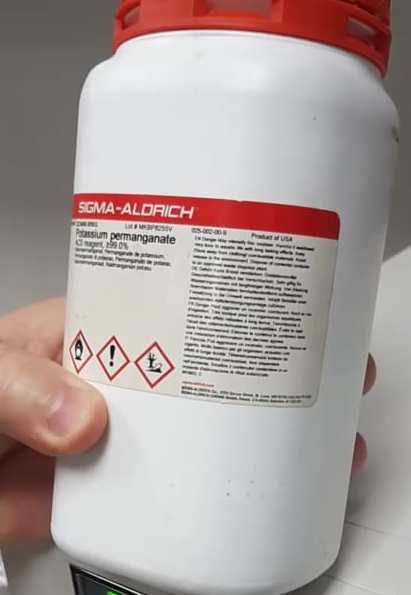
\includegraphics[width=0.3\textwidth]{Tarea1/muestras.png}
    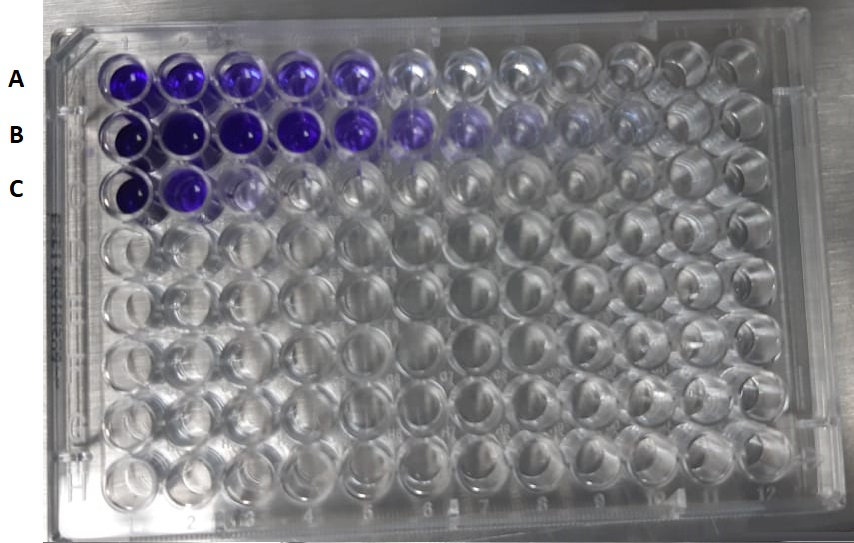
\includegraphics[width=0.49\textwidth]{Tarea2/microplaca2.jpeg}
    \caption{\textbf{Microplaca para el análisis en el espectrofotómetro para mezclas de agua con tinte azul.}}
    \label{microplaca2}
\end{figure}

 %\begin{table}[h!]%[c]{| c |}
%\begin{table}[h!]
    %\centering
\textbf{Tabla 1: Mezcla A.}        

\begin{tabular}{|c|c|c|c|c|c|}
    \hline
    Radio & 1:10 & 1:20 & 1:30 & 1:40 & 1:50\\
    \hline
    Absorbancia & $1.331$ & $0.704$ & $0.450$ & $0.393$ & $0.293$ \\
    \hline\hline\hline
    Radio & 1:200 & 1:500 & 1:1000 & 0:1 & 0:1\\
    \hline
    Absorbancia & $0.083$ & $0.065$ & $0.064$ & $0.050$ & $0.038$\\
    \hline
\end{tabular}
    
\textbf{Tabla 2: Mezcla B.}
    
\begin{tabular}{|c|c|c|c|c|c|}
    \hline
    Radio & 1:2 & 1:4 & 1:8 & 1:16 & 1:32\\
    \hline
    Absorbancia & $3.551$ & $1.820$ & $0.902$ & $0.440$ & $0.229$\\
    \hline\hline\hline
    Radio & 1:64 & 1:128 & 1:256 & 0:512 & \\
    \hline
    Absorbancia & $0.134$ & $0.089$ & $0.074$ & $0.070$ &\\
    \hline
\end{tabular}

\textbf{Tabla 3: Mezcla C.}
    
\begin{tabular}{|c|c|c|c|c|c|}
    \hline
    Radio & 1:10 & $1:10^2$ & $1:10^3$ & $1:10^4$ & $1:10^5$\\
    \hline
    Absorbancia & $0.717$ & $0.106$ & $0.048$ & $0.042$ & $0.045$\\
    \hline\hline\hline
    Radio & $1:10^6$ & $1:10^7$ & $1:10^8$ & $0:10^9$ & \\
    \hline
    Absorbancia & $0.040$ & $0.043$ & $0.037$ & $0.049$ & \\
    \hline
\end{tabular}

    %\caption{\textbf{Primera prueba.}}
    %\label{primera_prueba}
%\end{table}
%\end{table}

\textbf{\textcolor{azul50}{Análisis de los resultados}}

Ya comprobado que los datos fueron obtenidos dentro del rango de limitaciones especificado en la teoría previa, pasamos a procesar en matlab2017b los valores de absorbancia obtenidas por el SkanIt.

Es fácil ver que los valores correspondiente a concentración 0:1 mostrados en la Tabla 1 corresponden al agua destilada sin mezclar con el tinte, valores que dan una medida de error del instrumento ya que este debería estar en $\approx 0.042\pm 0.01$ para $200~\mu l$ mientras que el instrumento da valores con errores máximos visualizados de $\approx\pm 0.09$.

\begin{figure}
    %\centering
    %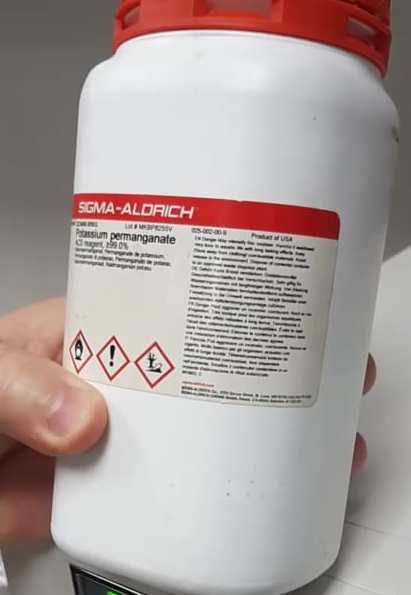
\includegraphics[width=0.3\textwidth]{Tarea1/muestras.png}
    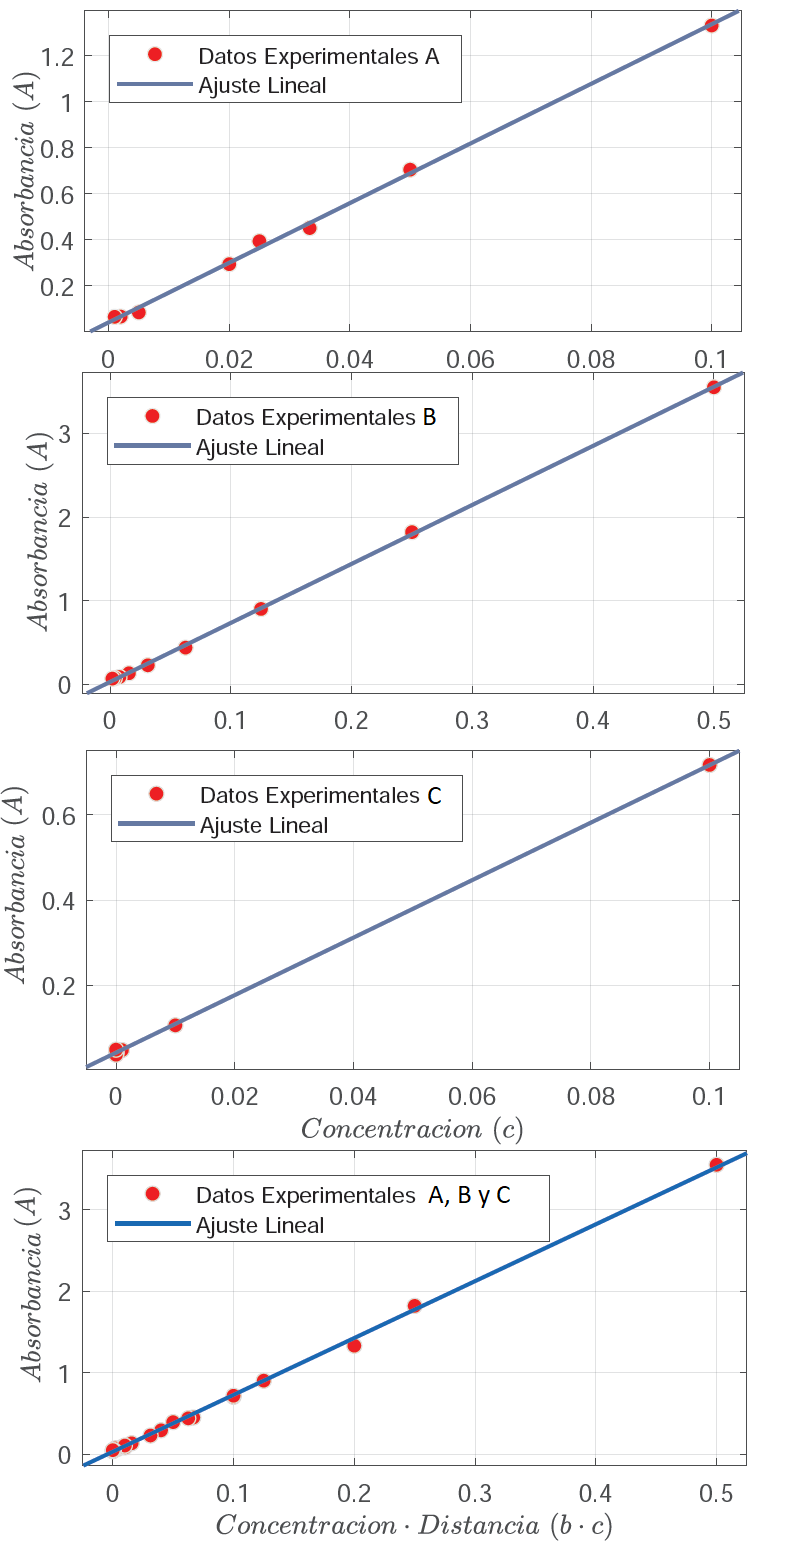
\includegraphics[width=0.49\textwidth]{Tarea2/absorbancia.png}
    \caption{\textbf{Análisis de los resultados de la Tabla 1, 2 y 3.}}
    \label{fig2.1}
\end{figure}

Con los datos mostrados en la Tabla 1, 2 y 3 se procesará a trabajar con los datos en la búsqueda de una tendencia empírica como la predicha por la Ley de Lambert y Beer mostrada en la ec. (\ref{ley}), para esto primeramente se grafeicará la $Absorbancia (A)~ vs~ Concentracion (c)$ y se ajustaran linealmente (a una ecuación de tipo $y~=~a\cdot x$) haciendo uso del Matlab~R2017b~(Ver~Fig.~\ref{fig2.1}).

Como resultado del ajuste lineal de estos datos experimentales tenemos valores de $R-square$ de $\approx 0.9983$, $\approx 0.9997$ y $\approx 0.9997$ para los datos de la Tablas 1, 2 y 3 o las mezclas A, B o C respectivamente, estos valores tan cercarnos a la unidad evidencian la correspondencia predicha por la ec. (\ref{ley}).

Con la intención de generalizar los resultados obtenidos se incluirán todos los mostrados en las Tablas 1, 2 y 3 en un gráfico de Absorbancia (A) vs Concentración $\cdot$ Distancia ($b\cdot c$) como los mostrados en la Fig. \ref{fig2.1}, la distancia del haz monocromático es proporcional a los $\mu l$ finales de las mezclas ($200~\mu l$, $100~\mu l$ y $90~\mu l$ respectivamente). Al realizar el respectivo ajuste lineal resulta en un $R-square \approx 0.9987$ reafirmando también su correspondencia con la ley de de Lambert y Beer.


\textbf{\textcolor{azul50}{Conclusiones}}

Se trabajó con la pipeta de laboratorio para muestras con diferentes proporción entre tinte azul y agua, estás fueron caracterizadas por un espectrofotómetro con un haz de luz monocromático y se comprobó su correspondencia con la Ley de Lambert y Beer, los valores de ajuste obtenidos por el Matlab R2017b comprobarón que el trabajo de laboratorio fue satisfactorio y la manipulación de las pipetas fue la adecuada.
























